\documentclass[12pt]{article}
\parindent0em
\parskip 1ex plus 0.4ex minus 0.4ex

\usepackage[a4paper,vmargin=30mm,hmargin=25mm]{geometry}
\usepackage{polyglossia}
\setdefaultlanguage{german}
\usepackage{fontspec}
\usepackage{lipsum}
\usepackage{xcolor}
\usepackage{listings}
\usepackage{amssymb}
\usepackage{hyperref}
\usepackage{graphicx}

\definecolor{lstbackground}{rgb}{0.95,0.95,1}      % hellgruener Rahmen
\lstset{language=Python}

\lstset{
  basicstyle=\small\ttfamily,
  backgroundcolor=\color{lstbackground},
  keywordstyle=\bfseries\ttfamily\color{blue},
  stringstyle=\color{orange!50!black}\ttfamily,
  commentstyle=\color{gray}\ttfamily,
  showstringspaces=false,
  flexiblecolumns=false,
  tabsize=4,
  numbers=left,
  numberstyle=\tiny,
  numberblanklines=true,
  stepnumber=1,
  numbersep=10pt,
  xleftmargin=15pt,
  literate=%
  {Ö}{{\"O}}1
  {Ä}{{\"A}}1
  {Ü}{{\"U}}1
  {ß}{{\ss}}1
  {ü}{{\"u}}1
  {ä}{{\"a}}1
  {ö}{{\"o}}1
  {~}{{\textasciitilde}}1
}

\begin{document}

\begin{center}
  \textbf{\LARGE Sichere Programmierung} \\[1ex]%
  \textbf{\Large Projekt 2}\\[2ex] %
  Julian Sobott \\ %
  (76511) \\ %
  David Sugar \\ %
  (76050) \\ %
  
\end{center}

% ****************************************************************************
\section{Zu Aufgabe 1}
% ****************************************************************************
\subsection{a)}
Zu beginn der \texttt{main()} Funktion wird eine \texttt{unsigned int} Variable, i, deklariert, jedoch nicht initialisiert, d.h. bis auf wenige Ausnahmen $i \in \{0..2^{32}-1\}$.

Danach wird die Variable im Kopf der darauf folgenden For-Schleife mit 0 initialisiert. Die Schleife inkrementiert die Variable i am Ende jedes Schleifendurchlaufs und tritt erneut in die Schleife ein, solange i kleiner 20 ist.
Innerhalb der Schleife wird der Wert von i, zum jeweiligen Zeitpunkt, formatiert mithilfe von \texttt{printf()} in der Standardausgabe ausgegeben. Dabei werden immer 2 Stellen ausgegeben, dies wird über \texttt{"\%2d"} realisiert.

\textbf{Potentielles Problem: Es sollte \texttt{"\%2u"} verwendet werden, da \texttt{d} für die Formatierung von signed Integern verwendet wird.} In diesem Fall spielt die Formatierung aber keine Rolle.

\subsection{b)}
Bild \ref{fig:aufgabe1b} zeigt die Ausgabe des Programms.
\begin{figure}[h]
	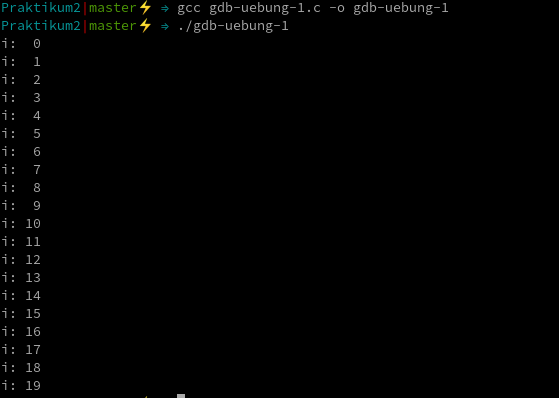
\includegraphics[scale=0.9]{Pictures/aufgabe1b.png}
	\caption{Ausgabe von gdb-uebung-1.c}
	\label{fig:aufgabe1b}
\end{figure}

\subsection{c)}
\begin{lstlisting}
	<+8>:	mov    DWORD PTR [rbp-0x4],0x0
    <+15>:	jmp    0x40113b <main+41>
    <+17>:	mov    eax,DWORD PTR [rbp-0x4]
    <+20>:	mov    esi,eax
    <+22>:	mov    edi,0x402004
    <+27>:	mov    eax,0x0
    <+32>:	call   0x401030 <printf@plt>
    <+37>:	add    DWORD PTR [rbp-0x4],0x1
    <+41>:	cmp    DWORD PTR [rbp-0x4],0x13
    <+45>:	jbe    0x401123 <main+17>
\end{lstlisting}

Für die Variable i wird Speicher auf dem Stack alloziert, die Anfangsadresse ist dabei \texttt{rbp-0x4}.

In Zeile <+8> wird i mit 0x0 initialisiert. Danach springt das Programm unbedingt in Zeile <+41>. Hier befindet sich nun die Überprüfung, ob die Schleife verlassen wird, d.h. $ i \ge 0x14 $, oder ein weiterer Schleifendurchlauf gestartet wird. Dazu wird in Zeile <+41> i mit 0x13 verglichen. Ist der Wert kleiner oder gleich 0x13 wird in Zeile <+17> gesprungen und damit ein weiterer Schleifendurchlauf gestartet. Andernfalls wird die nächste Instruktion ausgeführt und damit die Schleife verlassen.

In Zeile <+17> und <+20> wird der Wert von i, vom Speicher in das \texttt{esi} Register geladen. In der darauf folgenden Zeile wird die Adresse des Formatierungsstrings ("i: \%2d\\n") ( 0x402004 ) in \texttt{edi} geladen.

\begin{lstlisting}
gef➤  x/s 0x402004
0x402004:	"i: %2d\n"
\end{lstlisting}

Weiterhin wird \texttt{eax} wieder auf 0x0 zurückgesetzt. Danach wird \texttt{printf()} mit den in \texttt{edi} und \texttt{esi} geladenen Parametern aufgerufen. Schlussendlich wird i inkrementiert und daraufhin wieder verglichen (<+41>).

\subsection{•}






\end{document}



%%% Local Variables: 
%%% TeX-PDF-mode: t
%%% TeX-master: t
%%% coding: utf-8
%%% mode: latex
%%% TeX-engine: xetex
%%% End: 
